\documentclass[conference]{IEEEtran}
\IEEEoverridecommandlockouts

\usepackage{cite}
\usepackage{amsmath,amssymb,amsfonts}
\usepackage{graphicx}
\usepackage{booktabs}
\usepackage{multirow}
\usepackage{array}
\usepackage{textcomp}
\usepackage{xcolor}
\usepackage[hidelinks]{hyperref}

\newcommand{\oos}{\textsc{oos}}
\newcommand{\pts}{\,pts}

\begin{document}

\title{Automated Design of Task-Specific Intent and Slot Pipelines with a Small Language-Model Agent: A Controlled Evaluation on MASSIVE}

\author{
\IEEEauthorblockN{Mihir Bhati\IEEEauthorrefmark{1}}
\IEEEauthorblockA{\textit{School of Computer Science}\\
\textit{and Engineering}\\
\textit{Vellore Institute of Technology}\\
Chennai, India\\
24BCE5341\\
% TODO: add Mihir's email
email@vitstudent.ac.in}
\and
\IEEEauthorblockN{Ahana Sharan\IEEEauthorrefmark{1}}
\IEEEauthorblockA{\textit{School of Computer Science}\\
\textit{and Engineering}\\
\textit{Vellore Institute of Technology}\\
Chennai, India\\
24BCE5334\\
ahana.sharan2024@vitstudent.ac.in}
\and
\IEEEauthorblockN{Vijayaprabakaran K}
\IEEEauthorblockA{\textit{School of Computer Science}\\
\textit{and Engineering}\\
\textit{Vellore Institute of Technology}\\
Chennai, India\\
% TODO: add the guide's email
email@vit.ac.in}
\thanks{\IEEEauthorrefmark{1}Equal contribution.}
}

\maketitle

\begin{abstract}
Building the intent and slot component of a new assistant still requires a developer to decide, by trial and error, how the language model is prompted, which examples it sees and how it rejects unsupported requests. We present an agent that makes them from a project specification: a description, an intent inventory, an entity schema and ten labelled utterances per intent. The agent validates and enriches the specification, ranks the options of each design factor, evaluates four of twelve candidate pipelines on 100 development utterances, revises one factor, selects under schema-validity, entity and latency constraints, and exports a hash-verified package. Every planning and runtime call uses one 3-billion-parameter model running on a laptop. On three projects built from MASSIVE, one held out until the protocol was frozen, the agent chose the development-optimal design every time. Against a generic prompt it raised test intent macro-F1 by 2.2 and 4.9 points and entity F1 by 7.3 and 5.5 points on the two development projects, meeting the preregistered success rule; on the held-out project intent F1 fell by 1.3 points (not significant) while entity F1 rose by 14.6 points. It also scored above a k-shot XLM-R baseline on all three projects.
\end{abstract}

\begin{IEEEkeywords}
natural language understanding, intent classification, slot filling, out-of-scope detection, language model agents, in-context learning, automated pipeline design
\end{IEEEkeywords}

%=====================================================================
\section{Introduction}
%=====================================================================

A task-oriented assistant turns an utterance such as \emph{``wake me up at seven tomorrow''} into an intent (\texttt{alarm\_set}) and slot values (\texttt{time}\,=\,``seven'', \texttt{date}\,=\,``tomorrow''), and it must refuse requests it was not built for. Every new product has its own inventory: a smart-home controller, a calendar and e-mail helper and a food-ordering service share almost no intents. Fine-tuned encoders handle this well when labelled data is plentiful~\cite{chen2019bert,conneau2020unsupervised}, but plentiful means thousands of utterances. In MASSIVE~\cite{fitzgerald2023massive}, the alarm and smart-home domains alone contribute 1{,}159 training utterances, and a developer starting a new project rarely has them.

Small instruction-tuned language models (LMs) remove the training step. A 3-billion-parameter model quantised to 4 bits runs on a laptop GPU with 4\,GB of memory, answers in under half a second and can follow a label inventory from a handful of examples. What it does not remove is design work. The developer still has to decide whether intent and slots are requested in one call or two, whether the prompt describes each label, which demonstrations go into the prompt, and whether out-of-scope (\oos) requests are rejected by the model or by a similarity threshold. These choices matter. With the model and data held fixed, the twelve combinations we study span 13.5 points of development intent macro-F1 on one project (0.839 to 0.974) and 16.0 points on another (0.738 to 0.898).

Work on automating LM use has concentrated on rewriting instruction text~\cite{zhou2023large,pryzant2023automatic,yang2024large}, tuning the demonstrations of a fixed program~\cite{khattab2024dspy}, or replacing the LM with a fine-tuned small model~\cite{viswanathan2023prompt2model}. None of these produces a joint intent and span output with a rejection decision under deployment constraints, and they are rarely compared with random search at the same budget, the standard control for adaptive search~\cite{bergstra2012random}. Without that control, the contribution of the LM's reasoning cannot be separated from simply trying several options.

This paper asks whether an LM agent with a budget of four candidate evaluations can design an intent and slot pipeline that beats a generic prompt, random search, a human designer and a fine-tuned encoder trained on the same examples. The contributions are:
\begin{enumerate}
\item A formulation of task-specific NLU pipeline design as constrained selection over a factorised discrete design space, and an agent that analyses a project specification, plans, evaluates, revises, selects and exports a verifiable package (Section~\ref{sec:method}).
\item A factor-wise planning strategy that builds candidates one factor at a time and revises exactly one factor. It reached the best of the twelve designs on development data on all three projects with four evaluations, although the model's own first preferences were wrong on two of the three factors (Section~\ref{sec:trace}).
\item A controlled evaluation on three projects derived from MASSIVE, one of them held out until the protocol was frozen, against six baseline families including matched-budget random search, a human designer and fine-tuned XLM-R, with paired bootstrap confidence intervals (Section~\ref{sec:results}).
\end{enumerate}

%=====================================================================
\section{Literature Survey}
\label{sec:related}
%=====================================================================

This section focuses on an extensive survey of fifteen works that define the data, models, prompting methods and search procedures our system builds on.

\subsection{NLU datasets and fine-tuned models}

\emph{FitzGerald et al.}~\cite{fitzgerald2023massive} released MASSIVE, one million utterances in 51 languages localised by professional translators from the English SLURP corpus~\cite{bastianelli2020slurp}. Each utterance carries one of 60 intents across 18 scenarios and span annotations over 55 slot types. Their XLM-R and mT5 baselines are fine-tuned on the full training split. We use the English portion and restrict each project to a few scenarios, which yields small, realistic single-product inventories.

\emph{Larson et al.}~\cite{larson2019evaluation} built CLINC150, 150 intents over ten domains plus a separate set of queries that match none of them. They showed that classifiers with high in-scope accuracy recall few out-of-scope queries, whether rejection is done by a confidence threshold or by an extra ``out-of-scope'' class trained on examples. For this reason our design space treats rejection as a separate factor and we report \oos{} F1 separately.

\emph{Chen et al.}~\cite{chen2019bert} predicted the intent from BERT's sentence representation and the slot tags from its token representations, training both objectives together. On ATIS and Snips, joint training improved intent accuracy, slot F1 and whole-utterance accuracy over earlier recurrent and attention-based models. Joint encoders remain the reference architecture for intent and slot tasks, and our fine-tuned baseline follows the same two-head design.

\emph{Conneau et al.}~\cite{conneau2020unsupervised} trained XLM-R, a masked language model, on 2.5\,TB of filtered web text in 100 languages and reported strong cross-lingual transfer on classification, question answering and named entity recognition. We fine-tune its base version on the ten utterances per intent the agent sees and on each project's full training split.

\subsection{In-context learning and example selection}

\emph{Brown et al.}~\cite{brown2020language} showed that a sufficiently large autoregressive LM can perform a new task from an instruction and a few demonstrations placed in its prompt, without any weight update, and that accuracy rises with the number of demonstrations and with model size. Once a task is specified through the prompt, its contents and the number of calls become design decisions, which our design space enumerates.

\emph{Liu et al.}~\cite{liu2022makes} retrieved, for each test input, the training examples nearest to it in a sentence-encoder space and placed them in the prompt. Nearest-neighbour demonstrations beat randomly sampled ones on sentiment analysis, table-to-text generation and open-domain question answering. Our similarity-based example selection applies the same idea with a lexical TF-IDF index, which costs nothing at request time and needs no second model.

\subsection{Automatic prompt and program optimisation}

\emph{Zhou et al.}~\cite{zhou2023large} proposed Automatic Prompt Engineer (APE): an LM writes candidate instructions from input--output pairs, each candidate is scored on held-out examples, and the best is kept or resampled. The generated instructions matched or exceeded human-written ones on most instruction-induction tasks tested. APE's output is a prompt, not a pipeline, for tasks with a single label or string as output.

\emph{Pryzant et al.}~\cite{pryzant2023automatic} described the errors of a prompt on a minibatch in natural language, treated that description as a ``gradient'', edited the prompt against it, and kept the best edits with beam search and a bandit procedure. The method improved initial prompts on several binary classification tasks. Our revision phase borrows the idea of showing the model an error report, but confines its answer to one move in a discrete space, so a wrong suggestion costs one evaluation and cannot produce an unrunnable pipeline.

\emph{Yang et al.}~\cite{yang2024large} cast optimisation as prompting (OPRO): the meta-prompt lists earlier solutions with their scores and the LM proposes a new one. They applied it to small regression and travelling-salesman instances and to instruction search on GSM8K and Big-Bench Hard. OPRO needs many proposal rounds; our setting allows one, because every candidate evaluation costs about a hundred model calls on development data.

\emph{Khattab et al.}~\cite{khattab2024dspy} introduced DSPy, in which an LM pipeline is written as declarative modules and a compiler bootstraps demonstrations and instructions to maximise a user-supplied metric. Compiled pipelines let small open models compete with larger prompted ones on multi-hop question answering and math word problems. DSPy optimises the contents of a structure the developer writes; our agent chooses the structure, including the number of calls per request and where rejection happens.

\subsection{From task description to deployable system}

\emph{Viswanathan et al.}~\cite{viswanathan2023prompt2model} built Prompt2Model, which takes a task description with a few examples, retrieves related datasets and a pretrained model, generates further training data with an LM and fine-tunes a small model for deployment. It is the closest work to ours in aim, a deployable artefact from a description, but it requires training and was not evaluated on slot filling or out-of-scope rejection.

\subsection{Agents and self-correction}

\emph{Madaan et al.}~\cite{madaan2023selfrefine} let one LM generate an output, criticise it and rewrite it, repeating until a stopping condition, with no training. The loop improved outputs on seven tasks including dialogue response and code optimisation. We use a narrow form of self-correction at runtime: when an output breaks the schema, the model receives the specific violation and one chance to repair it.

\emph{Yao et al.}~\cite{yao2023react} interleaved reasoning traces with actions such as search queries, so that observations from the environment inform the next reasoning step. ReAct improved question answering and fact verification and reduced hallucination compared with reasoning alone. Our agent follows the same pattern at the level of design: it reasons, acts by running a candidate on development data, observes the scores and error report, and acts once more.

\subsection{Search baselines and automated machine learning}

\emph{Bergstra and Bengio}~\cite{bergstra2012random} showed that random search finds good hyper-parameters with far fewer trials than grid search, because only a few dimensions usually matter. Random search has since become the baseline any adaptive optimiser must beat at an equal budget. We therefore compare the agent with five seeds of random search over the same twelve designs, with the same four-evaluation budget and the same selection rule.

\emph{He et al.}~\cite{he2021automl} surveyed automated machine learning across data preparation, feature engineering, hyper-parameter optimisation and neural architecture search, and organised it by search space, search strategy and evaluation cost. In their terms our system is a pipeline-level AutoML method with a small hand-defined search space, an LM as the search strategy and development-set evaluation as the expensive step.

\subsection{Research gap}

Table~\ref{tab:related} compares the eight most relevant approaches. Prompt and program optimisers search instruction text or demonstrations for one output metric; fine-tuning approaches need training data and compute; none of them produces intent, character-level slots and a rejection decision together under schema and latency constraints. More importantly for an agent claim, only one of them compares its search with a random-sampling search of the same kind, and none does so for a complete pipeline, so the contribution of the LM's reasoning to pipeline design has not been isolated. The gap we address is therefore: \emph{whether a small local LM agent, given only a project specification and a fixed evaluation budget, chooses better complete intent and slot pipelines than random choice, a generic prompt and a human, when tested under a frozen protocol.}

\begin{table*}[t]
\centering
\caption{Comparison with the most relevant prior work}
\label{tab:related}
\resizebox{\textwidth}{!}{%
\begin{tabular}{@{}llccccc@{}}
\toprule
Work & What is searched or learned & Labelled data needed & Slot spans & \oos{} rejection & Deployable artefact & Random-search control \\
\midrule
Chen et al.~\cite{chen2019bert} & encoder weights & full training set & yes & no & model & -- \\
FitzGerald et al.~\cite{fitzgerald2023massive} & encoder weights (XLM-R, mT5) & full training set & yes & no & model & -- \\
Liu et al.~\cite{liu2022makes} & demonstrations per input & training pool & no & no & no & random examples \\
Zhou et al.~\cite{zhou2023large} & instruction text & few examples & no & no & prompt & no \\
Pryzant et al.~\cite{pryzant2023automatic} & instruction text & small labelled set & no & no & prompt & Monte-Carlo sampling \\
Yang et al.~\cite{yang2024large} & instruction text & small labelled set & no & no & prompt & no \\
Khattab et al.~\cite{khattab2024dspy} & demonstrations and instructions & small labelled set & no & no & compiled program & no \\
Viswanathan et al.~\cite{viswanathan2023prompt2model} & data and model weights & few examples & no & no & small model & no \\
\midrule
\textbf{This work} & \textbf{pipeline design (3 factors)} & \textbf{10 per intent + 100 dev} & \textbf{yes} & \textbf{yes} & \textbf{hashed package} & \textbf{yes, 5 seeds} \\
\bottomrule
\end{tabular}}
\end{table*}

%=====================================================================
\section{Proposed Methodology}
\label{sec:method}
%=====================================================================

\subsection{Problem formulation}

A project is a tuple $P=(D,I,E,K,C)$. $D$ is a free-text description of the product. $I$ is the intent inventory and $E$ the entity schema, which lists the entity types and, for each intent, the types that intent may carry. $K$ is a pool of labelled utterances with $k=10$ per intent, each annotated with its intent and entity spans. $C$ holds the deployment constraints: a minimum schema validity $S_{\min}$, a minimum entity F1 relative to a reference and a maximum 95th-percentile latency $L_{\max}$. A labelled development set $V$ contains in-scope utterances and \oos{} utterances drawn from unrelated domains.

A pipeline maps an utterance $u$ either to a rejection or to a pair $(\hat{\imath}, \hat{S})$, where $\hat{\imath}\in I$ and $\hat{S}$ is a set of typed character spans of $u$. The task is to choose a pipeline design $\theta$ from a design space $\Theta$ that performs best on unseen requests, while evaluating at most $B=4$ designs on $V$ and satisfying $C$.

\begin{figure*}[t]
\centering
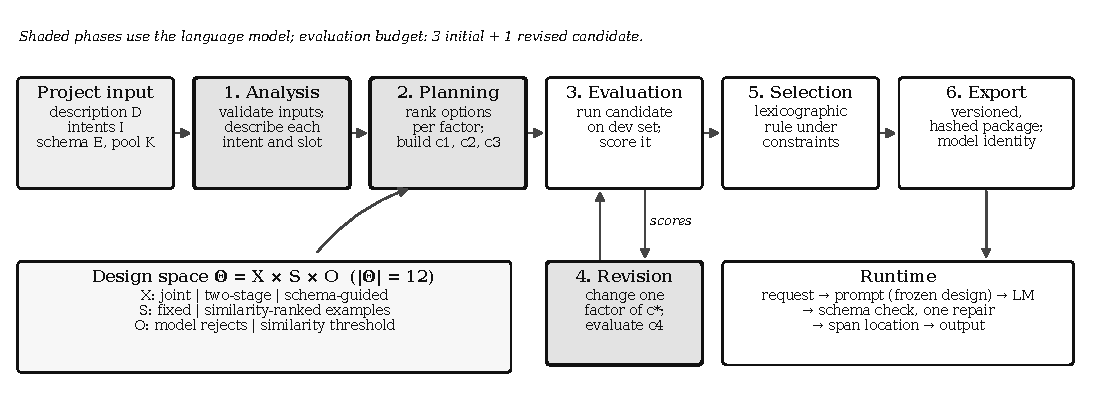
\includegraphics[width=\textwidth]{figures/architecture.pdf}
\caption{System architecture. The project specification passes through six phases; the shaded phases call the language model. Evaluation and revision form one loop with a hard budget of three initial candidates and one revised candidate. The exported package is executed by the runtime path on the right.}
\label{fig:arch}
\end{figure*}

\subsection{Design space}

$\Theta = X \times S \times O$ has three factors and $3\times2\times2=12$ designs. Every design is a fixed, trusted component; the agent chooses among them and never generates executable code.

\emph{Extraction strategy} $X$. \textbf{Joint}: one call returns the intent and all entities. \textbf{Two-stage}: the first call returns only the intent; the second asks only for the entity types that intent carries, with demonstrations of that intent, so each request costs two calls. \textbf{Schema-guided}: one call, but the prompt gives a one-line description of every intent and entity type.

\emph{Example selection} $S$. \textbf{Fixed}: one demonstration per intent, identical for every request. \textbf{Similarity}: the $m=16$ pool utterances nearest to the request by cosine similarity of word unigram and bigram TF-IDF vectors,
\begin{equation}
\mathrm{sim}(u,x)=\frac{\phi(u)^{\top}\phi(x)}{\lVert\phi(u)\rVert\,\lVert\phi(x)\rVert},
\end{equation}
where $\phi$ is the TF-IDF map fitted on $K$ with sublinear term frequency.

\emph{Rejection policy} $O$. \textbf{Model label}: the label \texttt{none\_of\_the\_above} is offered in the prompt and the model may choose it. \textbf{Threshold}: the request is rejected before any model call when $\max_{x\in K}\mathrm{sim}(u,x)<\tau^{*}$. The threshold is tuned on $V$ only,
\begin{equation}
\tau^{*}=\arg\max_{\tau\in\mathcal{T}} \; F_1^{\text{macro}}\!\left(I\cup\{\oos\};\,\tau\right),
\end{equation}
where $\mathcal{T}$ is the set of observed similarity values, so the search covers every distinct decision, and ties go to the lower threshold, which rejects fewer in-scope requests.

All designs share a prompt limit of 16 demonstrations and 2{,}000 input tokens. When the limit is reached, demonstrations are removed first; label definitions are never truncated.

\subsection{Phase 1: specification analysis}

Analysis has a deterministic validation part and an LM enrichment part. Validation checks the specification for duplicate or conflicting names, pool utterances labelled with undeclared intents or entity types, intents with fewer than $k$ examples and entity types that never occur in the pool. A conflict stops the run; the coverage findings are passed on to planning. Enrichment uses two LM calls to write a one-line description for every intent and every entity type. The LM may only describe names that already exist: a description of an unknown name is discarded and a missing one is reported rather than invented, so the supplied schema always takes precedence over model output. The schema-guided strategy places these descriptions in its prompts.

\subsection{Phase 2: candidate planning}

The planner receives the description, the size of the inventory, the coverage findings and a short neutral guide to each factor. We study two planners with the same budget.

\emph{Direct planner (A1).} The LM is asked to name three designs from the catalogue. Any name not in the catalogue is replaced from a fixed order that spreads the three extraction strategies, and each choice is recorded as reasoned or fallback.

\emph{Factor-wise planner (A2).} One LM call ranks the options of each factor separately and gives one reason per factor, producing orders $x_1\succ x_2\succ x_3$, $s_1\succ s_2$ and $o_1\succ o_2$. The three initial candidates are
\begin{equation}
c_1=(x_1,s_1,o_1),\quad c_2=(x_1,s_2,o_1),\quad c_3=(x_2,s_1,o_1).
\end{equation}
Whatever the model prefers, the alternative example selection and the runner-up extraction strategy are each measured once against its top choice. A malformed ranking for a factor falls back to the declared option order and the candidates are then marked as fallback.

\subsection{Phase 3: evaluation}

Each candidate runs on all of $V$ and is scored with the metrics of Section~\ref{sec:metrics}. The phase also writes an error report that lists, for every candidate evaluated so far, its intent macro-F1, entity F1, the fraction of valid replies, the fraction of in-scope requests wrongly rejected and the fraction of predicted entity values not found in the utterance.

\subsection{Phase 4: revision}

Let $\hat{c}$ be the best candidate so far under the selection rule below. Its neighbourhood
\begin{equation}
N(\hat{c})=\{\,c\in\Theta \setminus \mathcal{E} : c \text{ differs from } \hat{c} \text{ in exactly one factor}\,\}
\end{equation}
excludes the set $\mathcal{E}$ of designs already evaluated. The LM receives the error report and the list of moves in $N(\hat{c})$ and must choose one; an invalid reply falls back to the first move in a fixed factor order. The chosen design is evaluated as the fourth and last candidate. In A1 the revision may name any untried design. The four-evaluation cap is enforced by the agent, not left to the model.

\subsection{Phase 5: selection}

Let $\mathcal{C}$ be the evaluated candidates. The eligible set keeps those that meet every declared constraint,
\begin{equation}
\mathcal{C}_{\text{ok}}=\{c\in\mathcal{C}: \mathrm{SV}(c)\ge S_{\min},\ F_1^{E}(c)\ge f_{\min},\ \hat{L}_{95}(c)\le L_{\max}\},
\end{equation}
and the selected design maximises, in lexicographic order, intent macro-F1, then entity F1, then the negative latency estimate, with the design identifier as a final deterministic tie-break:
\begin{equation}
c^{*}=\arg\operatorname{lexmax}_{c\in\mathcal{C}_{\text{ok}}}\big(F_1^{\text{macro}}(c),\,F_1^{E}(c),\,-\hat{L}_{95}(c)\big).
\end{equation}
No weighted average is used, so a trade-off cannot be hidden in the weights. If $\mathcal{C}_{\text{ok}}$ is empty the agent reports that no candidate met the constraints instead of relaxing them. Cached development runs carry no timing, so $\hat{L}_{95}$ is an estimate from the number of calls per request; the latency of the selected design is measured afterwards without caching. The random-search baseline uses exactly the same rule, so the two differ only in which candidates they evaluate.

\subsection{Phase 6: export and runtime}

The package contains the frozen design, the enriched specification, the example pool, $\tau^{*}$, the prompt templates, the model's name and weights digest, and a SHA-256 hash of every file. Loading recomputes the hashes and refuses to run if any file or the model digest differs, so the deployed pipeline is provably the one that was evaluated.

At runtime a request follows the path at the right of Fig.~\ref{fig:arch}. Under the threshold policy it may be rejected immediately. Otherwise the prompt is built from the frozen design and sent to the LM at temperature zero with structured output. The reply must be an object whose intent is in $I$ or is \texttt{none\_of\_the\_above} and whose entities have declared types and string values. A violation triggers one repair call that states the specific error; a second failure is recorded as invalid and kept in every denominator.

The LM returns entity strings, not offsets, so a deterministic span-location rule converts them. Leading and trailing whitespace and quotation marks are removed; the string is searched in the utterance case-sensitively, then case-insensitively; with several matches the first occurrence not already claimed by another entity is taken. A string that does not occur is \emph{unsupported}: it counts as a false positive and is never fuzzy-matched. Every LM-based system in our evaluation uses this same rule.

\subsection{Evaluation metrics}
\label{sec:metrics}

Intent macro-F1 is computed over the in-scope requests and the project's intents:
\begin{equation}
F_1^{\text{macro}}=\frac{1}{|I|}\sum_{i\in I}\frac{2P_iR_i}{P_i+R_i},
\end{equation}
where $P_i$ and $R_i$ are the precision and recall of intent $i$. Rejecting an in-scope request, or returning an invalid output, counts as an error for its true intent. Entity F1 is micro-averaged over exact matches of (type, start, end) triples on in-scope requests: with gold spans $G$ and predicted spans $\hat{S}$,
\begin{equation}
P^{E}=\frac{|G\cap\hat{S}|}{|\hat{S}|},\quad R^{E}=\frac{|G\cap\hat{S}|}{|G|},\quad F_1^{E}=\frac{2P^{E}R^{E}}{P^{E}+R^{E}}.
\end{equation}
\oos{} F1 treats rejection as the positive class over all requests. Schema validity $\mathrm{SV}$ is the fraction of requests whose final output satisfies the contract after at most one repair. Latency is the median and 95th percentile of wall-clock time per request over uncached runs.

%=====================================================================
\section{Implementation and Result Analysis}
\label{sec:results}
%=====================================================================

\subsection{Dataset and projects}

We use the English (en-US) portion of MASSIVE~1.1~\cite{fitzgerald2023massive}, released under CC~BY~4.0: 16{,}521 utterances covering 18 scenarios, 60 intents and 55 slot types. Three projects were defined by grouping related scenarios (Table~\ref{tab:projects}). For each project, the pool $K$ takes ten utterances per intent from the official training split, the development set takes 80 in-scope utterances from the official development split, and the test set takes 250 from the official test split. Both add \oos{} utterances (20 and 50) drawn from eleven scenarios that belong to no project. P3's test set has 167 in-scope and 33 \oos{} utterances because its official test split holds only 181 in-scope utterances. Sampling used a fixed seed. The entity schema of each project was derived from its training split only, as a developer would declare it before seeing evaluation data; consequently five of P2's 26 entity types never appear in its pool and account for 10.7\% of its development gold entities.

\begin{table}[t]
\centering
\caption{The three projects built from MASSIVE en-US. Every development set has 80 in-scope and 20 \oos{} utterances.}
\label{tab:projects}
\small
\setlength{\tabcolsep}{4pt}
\resizebox{\columnwidth}{!}{%
\begin{tabular}{@{}llcccc@{}}
\toprule
Project & Scenarios & $|I|$ & $|E|$ & $|K|$ & Test \\
\midrule
P1 home assistant & alarm, iot & 12 & 18 & 120 & 250\,+\,50 \\
P2 productivity & calendar, email, lists & 10 & 26 & 100 & 250\,+\,50 \\
P3 ordering, travel & takeaway, transport & 6 & 19 & 60 & 167\,+\,33 \\
\bottomrule
\end{tabular}}
\end{table}

P3 was held out completely: its description was committed at the start, but every split, including development, was locked by a data-access object that raises an error until released with the hash of the freeze commit. All development used P1 and P2. The protocol, thresholds, budgets, every system's selected design and all code were then frozen in one commit, and only after that were the test sets and P3 released.

\subsection{Model and environment}

All LM calls, both for planning and at runtime, use Qwen2.5-3B-Instruct~\cite{qwen2024qwen25} quantised to 4 bits (Q4\_K\_M), served locally by Ollama~0.40.2 on a laptop with an NVIDIA RTX~3050 GPU (4\,GB). Decoding uses temperature~0, seed~0, JSON-constrained output and at most 512 output tokens. Fifty repeated uncached requests gave 50 identical outputs, so a single run per configuration is deterministic. For prompts averaging 1{,}028 input tokens a single call took 0.42\,s at the median and 0.59\,s at the 95th percentile. Model replies are cached by prompt hash for reproducibility; cached replies never contribute a latency figure.

\subsection{Baselines}

\textbf{B0} is TF-IDF features with logistic regression trained on $K$, with an \oos{} threshold tuned on $V$; it predicts no entities. \textbf{B1} is a generic prompt: the joint, fixed-example, model-label design on the bare specification, i.e., what a developer gets without any design effort. \textbf{B2} is a human designer: a team member studied the development results through a worksheet and chose one design (38 minutes on P1; under 6 minutes on P2, assisted by a chat assistant, which we declare); B2 was not run on P3. \textbf{B3} fine-tunes XLM-R base~\cite{conneau2020unsupervised} with a joint intent and slot head, learning rate $3\times10^{-5}$ and batch size 16, either on $K$ for 30 epochs (B3-k) or on the full training split of the project's scenarios for 5 epochs (B3-full: 1{,}159, 3{,}180 and 828 utterances); its rejection threshold on maximum softmax probability is tuned on $V$. \textbf{B4-random} draws four designs uniformly at random and selects with the agent's rule, repeated with five seeds; \textbf{B4-best} evaluates all twelve designs and represents the best achievable choice on development data.

\subsection{Statistical protocol and success rule}

Differences between two systems are tested with a paired bootstrap over test utterances~\cite{koehn2004statistical}: 1{,}000 resamples with a fixed seed, both systems scored on the same resample, and the 2.5th and 97.5th percentiles of the difference as the 95\% interval. A difference is called significant when the interval excludes zero. The success rule was fixed before testing: an agent succeeds against B1 if intent macro-F1 improves by at least 2.0 points, entity F1 drops by at most 2.0 points, schema validity is at least 0.98, and test-time 95th-percentile latency is at most twice B1's measured in the same session. Latency was measured on 50 development requests per system after five warm-up requests, with the systems interleaved request by request so that any slowdown of the machine affects all of them equally.

\subsection{Overall results}

\begin{table*}[t]
\centering
\caption{Test results. Intent macro-F1 / entity span F1 / \oos{} F1. Best LM-based result per column in bold. B4-random reports the mean intent macro-F1 of five seeds, with the range.}
\label{tab:main}
\small
\setlength{\tabcolsep}{5pt}
\resizebox{\textwidth}{!}{%
\begin{tabular}{@{}lccc@{}}
\toprule
System & P1 home assistant & P2 productivity & P3 ordering and travel (held out) \\
\midrule
B0 TF-IDF + logistic regression & 0.699 / -- / 0.426 & 0.669 / -- / 0.403 & 0.769 / -- / 0.404 \\
B1 generic prompt & 0.876 / 0.626 / 0.875 & 0.823 / 0.477 / 0.662 & \textbf{0.895} / 0.529 / 0.771 \\
B2 human designer & 0.837 / 0.648 / 0.471 & 0.851 / 0.491 / 0.748 & not run \\
B3-k XLM-R, same 10 per intent & 0.809 / 0.650 / 0.568 & 0.800 / 0.461 / 0.536 & 0.770 / 0.515 / 0.505 \\
B3-full XLM-R, full training split & 0.883 / 0.802 / 0.604 & 0.904 / 0.775 / 0.560 & 0.913 / 0.721 / 0.581 \\
B4-random, mean (range) & 0.893 (0.881--0.903) & 0.854 (0.848--0.872) & 0.894 (0.882--0.909) \\
\midrule
A1 agent, direct planner & \textbf{0.903} / 0.639 / \textbf{0.885} & 0.852 / 0.504 / 0.758 & 0.889 / 0.506 / \textbf{0.845} \\
A2 agent, factor-wise planner & 0.898 / \textbf{0.699} / 0.865 & \textbf{0.872} / \textbf{0.532} / \textbf{0.767} & 0.882 / \textbf{0.675} / 0.795 \\
\bottomrule
\end{tabular}}
\end{table*}

Table~\ref{tab:main} and Fig.~\ref{fig:intent} give the test results. The selected designs were: A2 schema-guided with similarity examples and model rejection on P1 and P2, and joint with similarity examples and model rejection on P3; A1 two-stage with similarity examples on P1 and schema-guided with fixed examples on P2 and P3, all with model rejection. In each project A2's choice coincides with B4-best, the best of all twelve designs on development data.

\begin{figure}[t]
\centering
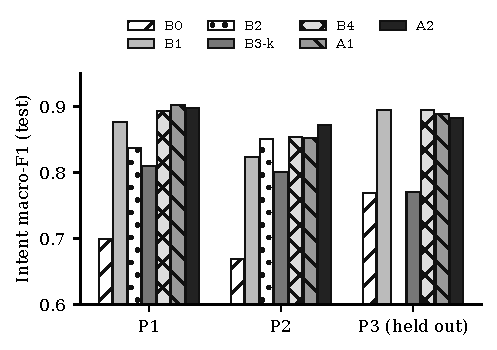
\includegraphics[width=\columnwidth]{figures/intent_test.pdf}
\caption{Test intent macro-F1. B4 is the mean of five random-search seeds. B2 was not run on P3.}
\label{fig:intent}
\end{figure}

\emph{Success rule.} Against B1, A2 changed intent / entity F1 by +2.2 / +7.3 points on P1, +4.9 / +5.5 on P2 and $-$1.3 / +14.6 on P3; A1 by +2.7 / +1.3, +2.9 / +2.7 and $-$0.6 / $-$2.3. Both agents therefore pass the rule on P1 and P2 and fail it on P3. Schema validity after repair was at least 0.997 in every agent run, and 95th-percentile latencies were within the limit (P1: A1 0.97\,s, A2 0.89\,s against 1.22\,s; P2: A1 0.77\,s, A2 1.08\,s against 1.67\,s). A2's median latency was 0.68\,s and 0.64\,s, against 0.45\,s and 0.41\,s for B1.

\emph{Significance.} Fig.~\ref{fig:ci} shows the paired intervals for intent macro-F1. A2's gain over B1 is significant on P2 (+4.9, 95\% CI [+1.1, +8.9]) but not on P1 (+2.2, [$-$0.6, +5.1]); on P3 the loss is not significant ($-$1.3, [$-$3.8, +1.4]). For entity F1, A2's gains over B1 are significant on all three projects: +7.3 [+0.8, +14.5] on P1, +5.5 [+0.3, +11.1] on P2 and +14.6 [+9.0, +21.3] on P3. None of A1's differences from B1 is significant. On test data 300 or 200 utterances give intervals about $\pm$3 points wide, so a two-point improvement, the threshold of the success rule, can pass the rule without being significant, as on P1.

\begin{figure}[t]
\centering
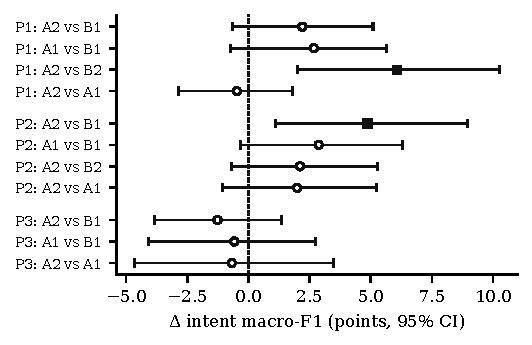
\includegraphics[width=\columnwidth]{figures/ci_test.pdf}
\caption{Paired bootstrap 95\% intervals of the difference in test intent macro-F1 (1{,}000 resamples). Filled squares: interval excludes zero.}
\label{fig:ci}
\end{figure}

\subsection{Agent against random search and the human designer}

Random search with the same budget and selection rule reached a mean intent F1 of 0.893, 0.854 and 0.894 on the three projects. A2 was above the mean on P1 (0.898) and P2 (0.872, the top of the random range), and at the bottom of the range on P3 (0.882). A random seed includes the development-optimal design among its four draws with probability $4/12$, and when it does, the shared selection rule picks it, so a seed can match A2 exactly. One of five seeds did so on P1 and P2, and two of five on P3. A2 reached that design on all three projects without depending on the draw.

Against the human designer, A2 was 6.1 points higher in intent F1 on P1 (95\% CI [+2.0, +10.2]) and 2.1 points higher on P2 (n.s.). On P1 the human chose the threshold rejection policy, which reduced \oos{} F1 to 0.471 against A2's 0.865; the agent never kept a threshold design because on both development projects all six model-label designs scored above all six threshold designs.

\subsection{Agent against fine-tuned encoders}

Trained on the same ten utterances per intent, XLM-R (B3-k) was 8.9, 7.2 and 11.2 points below A2 in intent F1 and below it in entity F1 on all three projects. Its rejection by maximum softmax probability gave \oos{} F1 between 0.505 and 0.568, against 0.767 to 0.865 for A2. With the full training split, 10 to 32 times more labelled data, XLM-R (B3-full) exceeded A2 in entity F1 by 4.6 to 24.3 points and in intent F1 on P2 and P3, but its \oos{} F1 stayed below 0.61. With a few examples per intent the LM pipeline is the better choice, and its rejection was better in every data condition tested; with thousands of annotated utterances a fine-tuned encoder extracts spans better.

\subsection{Why factor-wise planning worked}
\label{sec:trace}

Table~\ref{tab:trace} lists A2's four development candidates. On both P1 and P2 the planning model ranked fixed examples above similarity examples and the threshold policy above model rejection; on P1 its stated reason was that the threshold avoids model calls. Both preferences were wrong for these projects, and the first three candidates scored between 0.762 and 0.869. The construction of $c_2$ nevertheless measured similarity examples, which won, and the revision step, given the error report and the one-factor moves from $c_2$, switched its rejection policy to the model label. That single move raised development intent F1 by 10.5 points on P1 and 9.6 on P2 and reached the best of the twelve designs. A1, which names designs directly, began with B1's design on both projects, never combined schema guidance with similarity examples, and spent its unrestricted revision on a threshold design that scored 0.862 on P1 and 0.790 on P2; it stopped at 0.958 and 0.841. The gain comes from a structure that forces each factor to be tested and restricts revision to one-factor moves, not from better first guesses.

\begin{table}[t]
\centering
\caption{A2's development trace: intent macro-F1 / entity F1 of each candidate (100 development utterances)}
\label{tab:trace}
\small
\setlength{\tabcolsep}{3.5pt}
\resizebox{\columnwidth}{!}{%
\begin{tabular}{@{}llcc@{}}
\toprule
Step & Design & P1 & P2 \\
\midrule
$c_1$ & schema, fixed, threshold & 0.845 / 0.505 & 0.762 / 0.391 \\
$c_2$ & schema, similarity, threshold & 0.869 / 0.617 & 0.802 / 0.437 \\
$c_3$ & two-stage, fixed, threshold & 0.839 / 0.544 & 0.772 / 0.413 \\
$c_4$ & schema, similarity, model label & \textbf{0.974} / \textbf{0.707} & \textbf{0.898} / \textbf{0.483} \\
\midrule
\multicolumn{2}{@{}l}{Range over all 12 designs} & 0.839--0.974 & 0.738--0.898 \\
\bottomrule
\end{tabular}}
\end{table}

A2 was built after A1's development behaviour had been analysed, so its development scores on P1 and P2 are not independent evidence. Its test scores and all of P3 are: the design, the keep-or-drop rule and the code were frozen before either was released.

\subsection{Held-out project}

On P3 A2 again picked the best development design, joint extraction with similarity examples and model rejection, but on test it scored 1.3 points below B1 and at the bottom of the random-search range. The development set of P3 has 80 in-scope utterances over 6 intents, about 13 per intent, and the three designs selected by the random seeds lay within 2.7 points of each other on test (0.882 to 0.909), so the development ranking did not carry over to test. The entity gain carried over strongly: A2's entity F1 was 14.6 points above B1 and 16.9 points above A1 (CI [+10.7, +23.5]), because similarity-retrieved demonstrations show the model slot values like the ones in the request.

\subsection{Ablations}

Table~\ref{tab:ablation} removes one component of A1 at a time; each variant made its own choice on development data before testing. Removing selection (running the first candidate, which is B1's design) cost 2.7 and 2.9 points on P1 and P2, the largest effect, and gained 0.6 on P3. Removing the enrichment of analysis lowered P2 intent F1 by 1.1 and entity F1 by 7.4 points (0.504 to 0.430), consistent with P2's five entity types that never appear in the pool, for which the descriptions are the only information the model receives; this variant also chose a different design (two-stage with fixed examples). Removing the repair step changed intent F1 by at most 0.4 points, because the model rarely broke the schema.

\begin{table}[t]
\centering
\caption{Ablations of A1 on test, intent macro-F1}
\label{tab:ablation}
\small
\setlength{\tabcolsep}{5pt}
\begin{tabular}{@{}lccc@{}}
\toprule
Variant & P1 & P2 & P3 \\
\midrule
A1 (full) & 0.903 & 0.852 & 0.889 \\
without selection & 0.876 & 0.823 & 0.895 \\
without analysis enrichment & 0.903 & 0.841 & 0.898 \\
without planner reasoning & 0.903 & 0.848 & 0.882 \\
without schema repair & 0.907 & 0.852 & 0.889 \\
\bottomrule
\end{tabular}
\end{table}

\subsection{Cost and reproducibility}

Designing one project with A2 cost about 397 logical model calls: two for enrichment, two for planning and about 393 for running four candidates on 100 development utterances (two-stage designs need two calls per request, and threshold rejections need none), about a third of exhaustive evaluation and about three minutes of model time per project, against 38 minutes for the human designer on P1. Every reported metric was recomputed from the saved predictions of its run: 99 of 99 runs reproduced exactly, and an independent implementation of intent macro-F1, accuracy and \oos{} precision, recall and F1 agreed to nine decimal places. Retraining B0 from scratch reproduced all its test metrics exactly.

%=====================================================================
\section{Conclusion}
%=====================================================================

We built an agent that turns a project specification into a deployable, hash-verified intent and slot pipeline by evaluating four of twelve designs on 100 development utterances, using one 3-billion-parameter model on a laptop. Under a protocol frozen before the test data and the held-out project were seen, the factor-wise agent chose the development-optimal design on all three projects and met the preregistered success rule on both development projects, with intent gains of 2.2 and 4.9 points over a generic prompt. Its entity gains were significant on all three projects, including 14.6 points on the held-out project, where intent F1 fell by a non-significant 1.3 points. It scored above XLM-R trained on the same examples on every project. The gain came from planning that tests every factor and revises one at a time, not from the model's first preferences.

\section*{Acknowledgment}
The authors thank Vijayaprabakaran K for guidance throughout this work. MASSIVE is used under the CC~BY~4.0 licence. The human-designer baseline on P2 was assisted by a chat assistant, as stated in Section~\ref{sec:results}.
% TODO: add the AI-use statement your department requires for writing and code assistance.

\bibliographystyle{IEEEtran}
\bibliography{references}

\end{document}
